
\section{Appendix}

\subsection{General Compile Instructions}

I used the following software:
\begin{itemize}
    \item IPPL version: \texttt{V3.0.1}.
    \item Modules: \texttt{gcc/11.4.0}, \texttt{cmake/3.26.3}, \texttt{cuda/12.2.1}, \texttt{openmpi/4.1.4}.
    \item Tested GPU Architecture: GPX1050, PASCAL61.
    \item Used CPU: Intel Core i7-7700HQ (4 cores, 8 threads).
    \item Operating system: Windows 10, IPPL was used in the Linux Subsystem for Windows.
\end{itemize}
I used the \texttt{999-build-everything} script provided by IPPL to compile everything. For example:
\begin{verbatim}
    ippl-build-scripts/999-build-everything -t serial -k -f -i -u 
    ippl-build-scripts/999-build-everything -t openmp -k -f -i -u 
    ippl-build-scripts/999-build-everything -g PASCAL61 -t cuda -k -f -i -u 
\end{verbatim}
More instructions can be found in the GitHub repository with the code under \cite{aliemen2024}.

%TODO
%- Code is here...: 
%- Put code into folder: ....
%- Run like this and that for different testcases: ...
%- Used IPPL version 3.2.0, newer had problem with \texttt{hefte\_fft3d.h} and older didn't find Kokkos or somethin like that...
%- Coulomb logarithm: \url{https://farside.ph.utexas.edu/teaching/plasma/Plasma/node39.html}
%- Problem: only works for rho 1/NParticles in the beginning, even though later stages calculate NParticles/1...?!?!?!?!
%TODO


\subsection{Potential Problems and Bugs}

A list of potential problems and bugs:
\begin{itemize}
    \item There is a problem with applying the boundary conditions for very fast particles. When the boundaries are from $0$ to $L$ and the particle position is for example $>2*L$, then the particle will still not land inside the domain. Instead of calculating the modulo, only ``one domain size'' is subtracted. I fixed it by implementing my own boundary check in \texttt{applyExtendedBC()}.
\end{itemize}


\subsection{Old Cold Sphere Results}

For the presentation in the CSP lecture (FS24), we presented figure \ref{img:additional:disorder_heating_grid_comparison}. \\
\begin{minipage}[h]{\linewidth}
    \vspace{5pt}
    \centering
    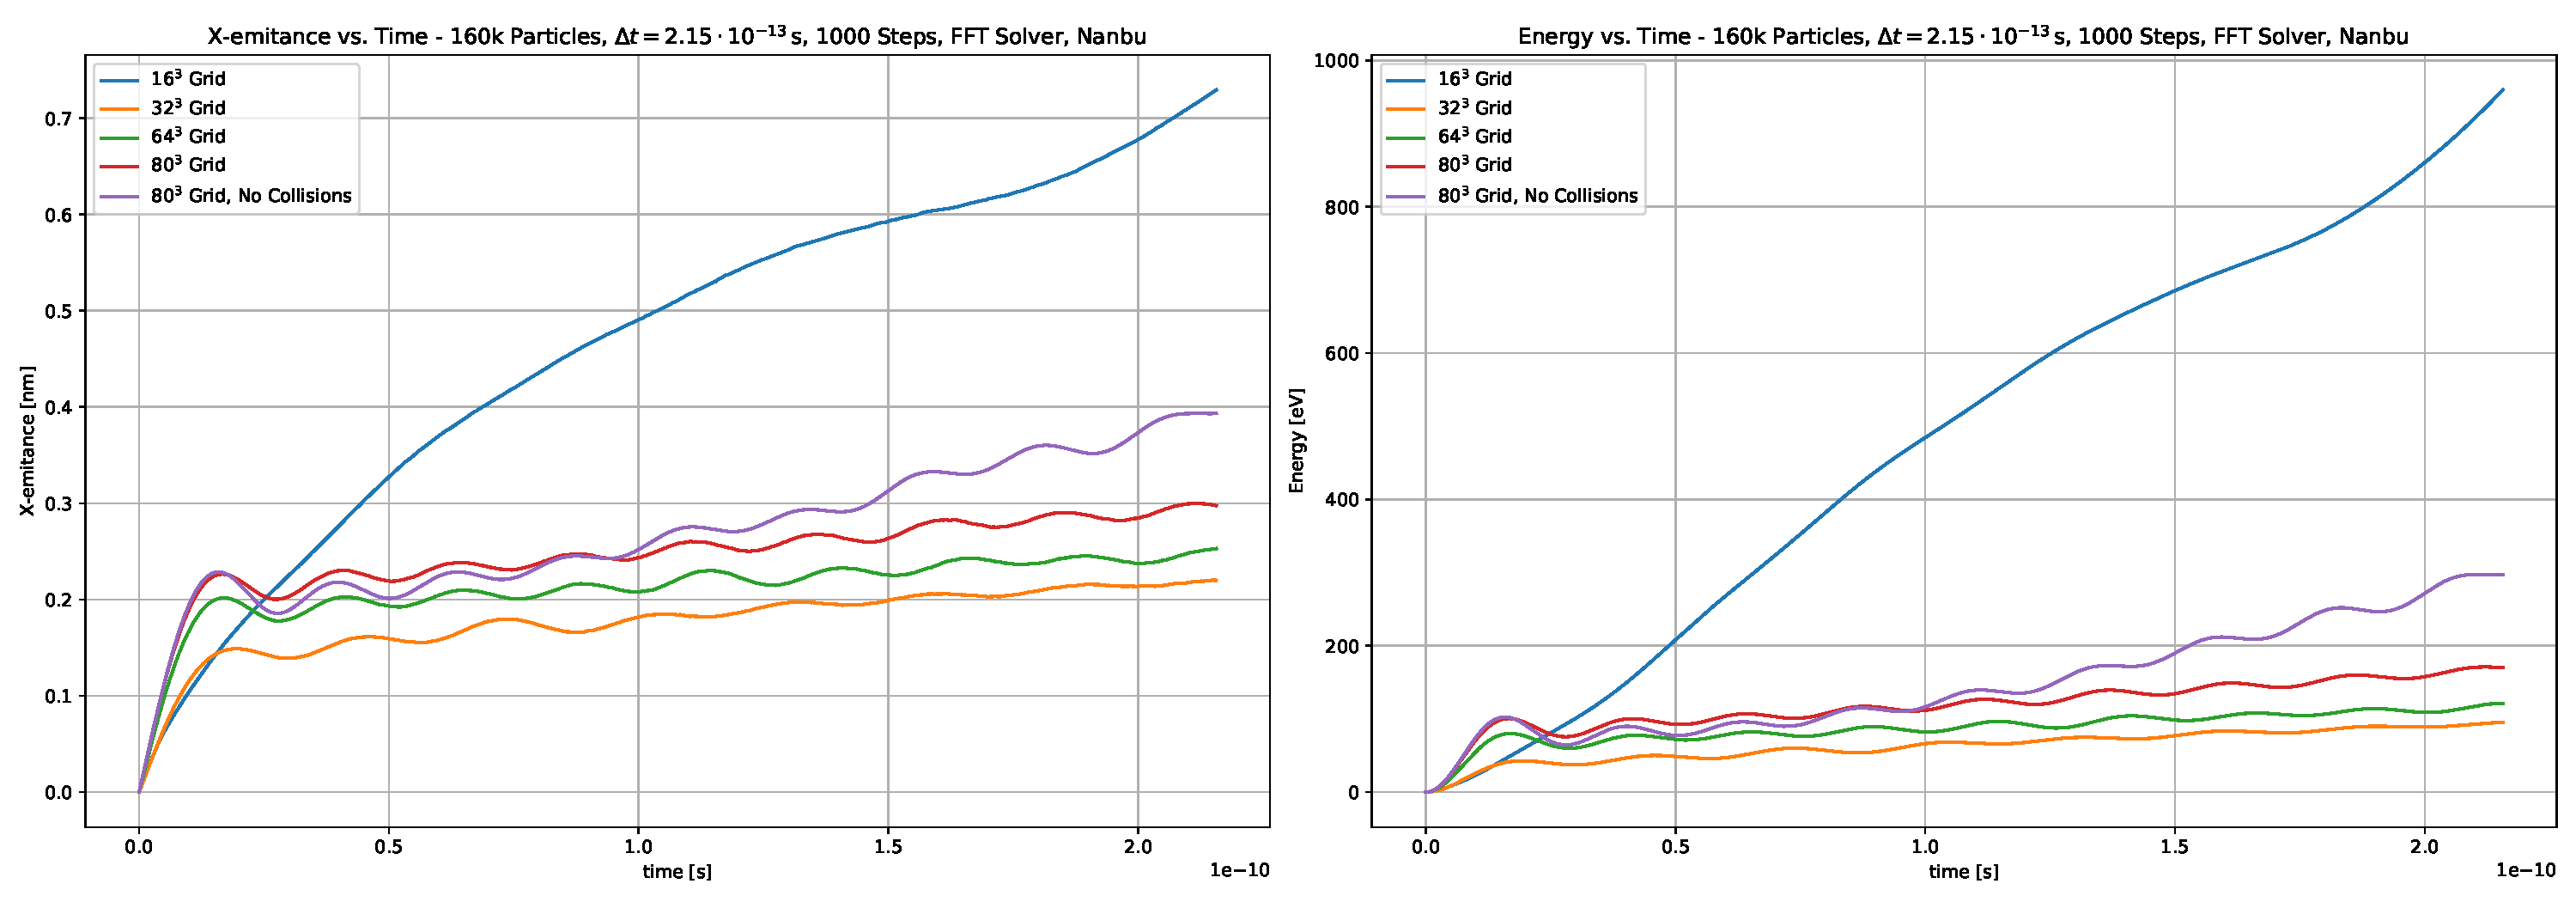
\includegraphics[width=\linewidth]{ressources/additional/disorder_heating_grid_comparison.pdf}
    \captionof{figure}{$x$-emittance and total energy against time for different mesh grid sizes.}\label{img:additional:disorder_heating_grid_comparison}
    \vspace{5pt}
\end{minipage}
The simulation was done using $156055$ particles and \textsc{Nanbu}'s collision algorithm.
